\chapter{Data visualisation}
\label{cha:visualisation}
Nodes in a network represent biological concepts ({\it{e.g.}} genes / proteins / metabolites) and biological interactions are modeled as links between them, {\it{i.e.}} relations between concepts ({\it{e.g.}} a gene encodes a protein).
Firstly, we will look at the basic user interface of Ondex.
Then we will load up a network to show the commonly used features and some of the core functionality such as layouts, annotators and filters. 

Help on starting Ondex is available in Section \ref{sec:ref_install}.
Once launched, you should see a window that looks like in Figure \ref{fig:launch_Ondex}.

\begin{figure}[H]
\centering
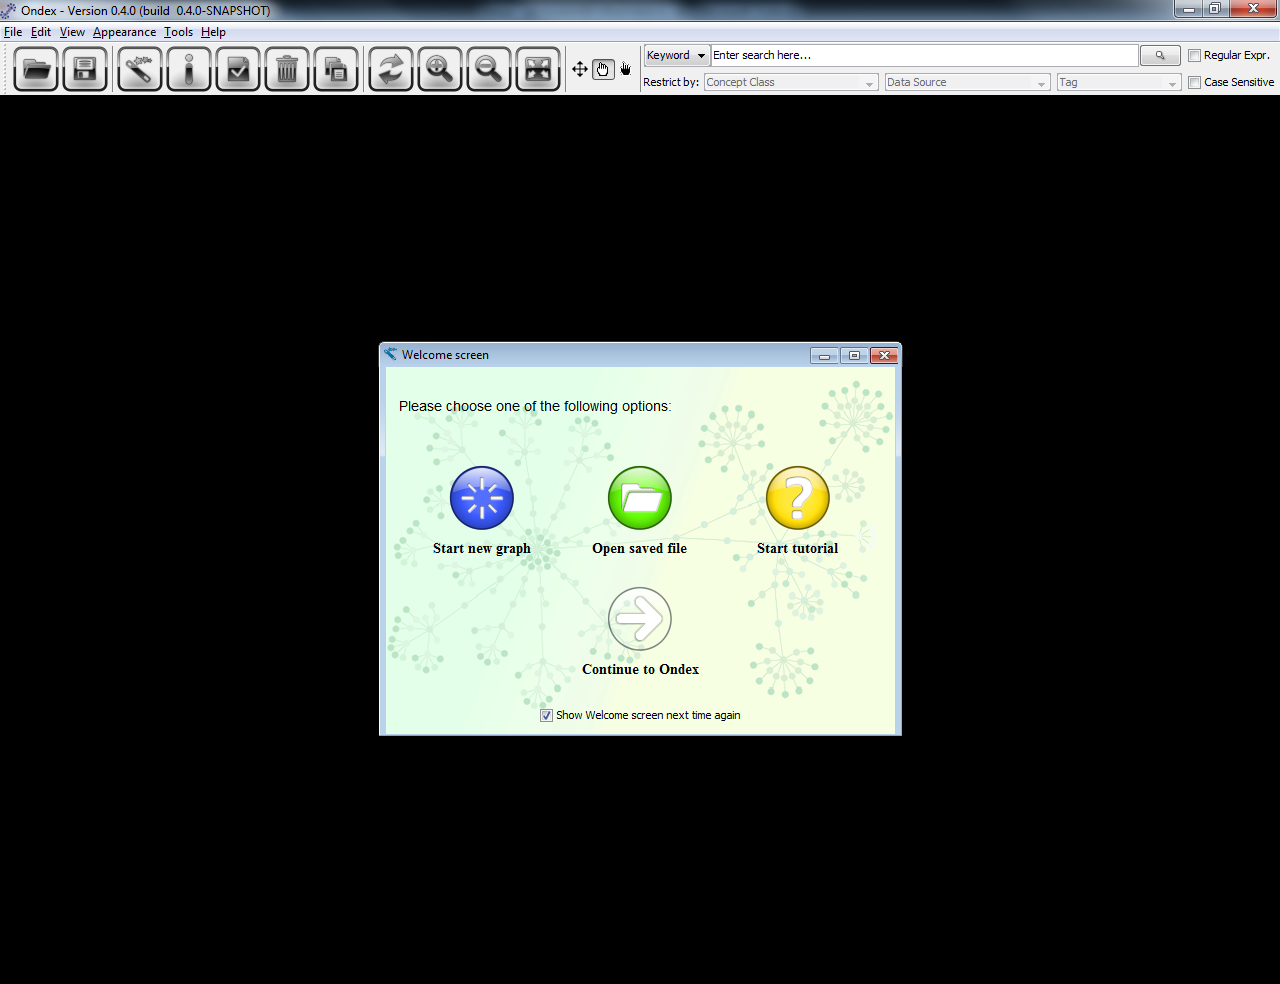
\includegraphics[scale=0.3]{images/Jun12/launched_Ondex.png}
\caption{Launching Ondex}
\label{fig:launch_Ondex}
\end{figure}

\begin{itemize}
\item At the top of the Ondex window there is a tool-bar which contains the menus, icons and search bar. 
Tool-tips are available for each icon when the mouse pointer hovers over it.
\item The rest of the window is used to show visualisation windows and pop-up dialog boxes to set up filters, annotators, etc.
\item When Ondex is launched, a welcome screen is displayed in the middle of the main window. 
This welcome screen window offers the users four buttons which are shortcuts to opening an empty network, opening an existing network, starting the tutorial or continuing to Ondex without taking any immediate action. 
Finally, at the bottom of the window, users are given the option of deselecting a check-box if they do not wish this welcome screen window to pop up automatically the next time Ondex is started.
\end{itemize}

%%%%%%%%%%%%%%%%%%%%%%%%%%%%%%%%%%%%%%%%%%%%%%%%%%%%%%%%%%%%%%%%%%%%%%%%%%%%%%%%%%%%%%%%%%%%%%%%%%%%%%%%%%%%%%%%%%%%%%%%%%%%%%%%%%%%%%%%%%%%%%%%%%%%%%%%%%
\section{Loading Networks and Basics}
\label{sec:loading}
We will now load a network (a subset of the AraCyc database) to show commonly used features of the user interface.
More information on loading and saving networks is available in Section \ref{sec:ref_loading}.
\begin{itemize}
\item Go to File -$>$ Open  (or click on the first button in the icon bar)
\item You should see an Open File Dialog
\item Open the Tutorial\_files/Main\_part folder, select aracyc\_subset.oxl and click on open
\end{itemize}
You should see the following:
\begin{figure}[H]
\centering
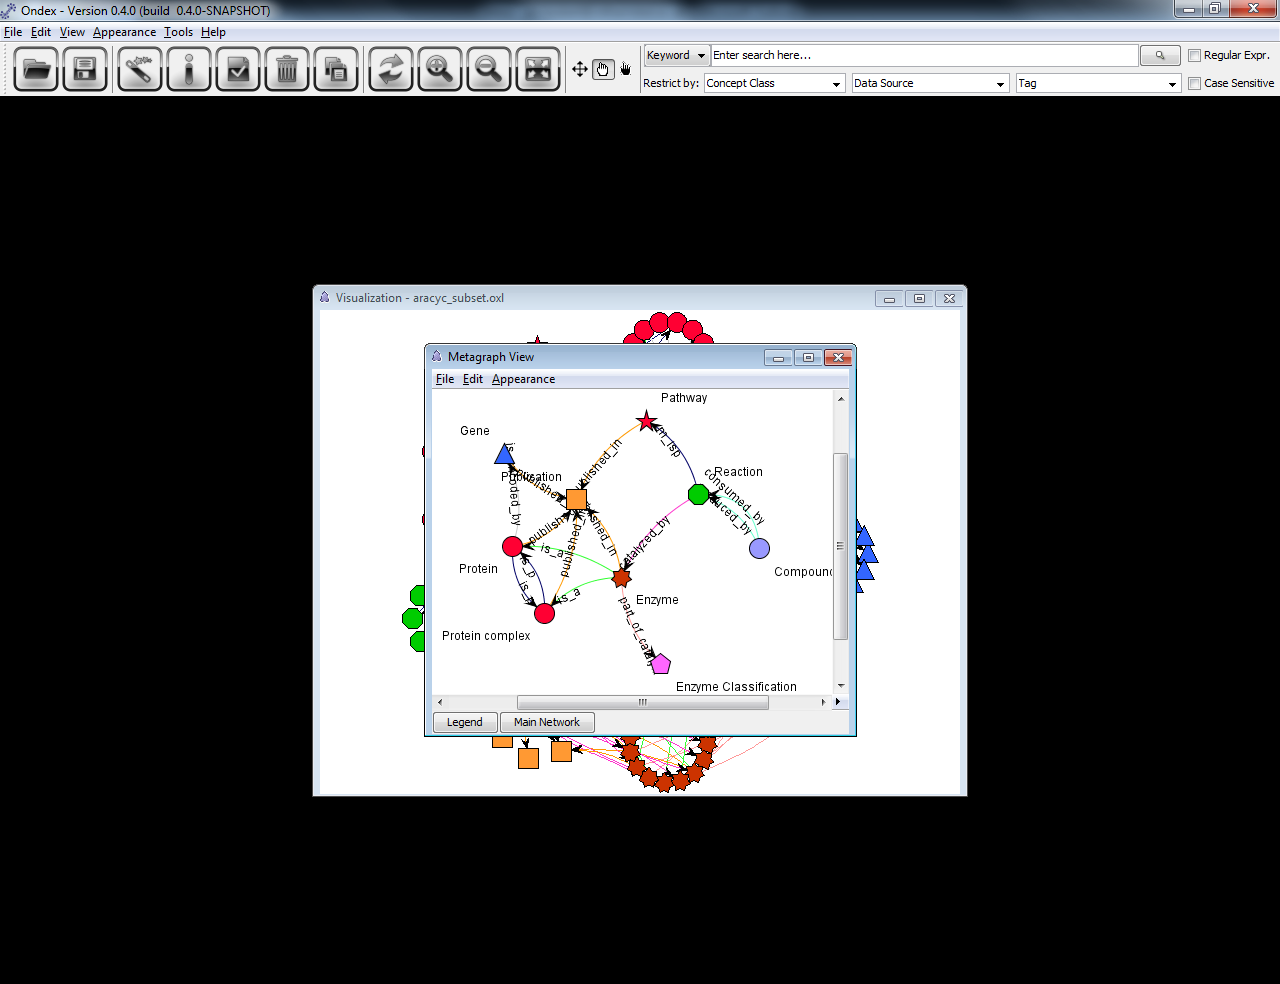
\includegraphics[scale=0.3]{images/Jun12/launched_aracyc_subset.png}
\caption{Metagraph - AraCyc}
\label{fig:metagraph_aracyc}
\end{figure}

The first window that shows is the ``Metagraph View''. Below this window is the main visualisation window for the network.
\emph{Note:} the main network will be minimized in the bottom left-hand side corner if the whole graph contains more than 2000 concepts or relations (in which case it is a good idea to filter it first, see Section \ref{sec:analysing}), otherwise it will appear behind the metagraph (as it is here). 

The metagraph gives an overview of all the different types of concepts present on the main network, as well as all the different types of relations which connect them.

The metagraph view has 2 buttons at the bottom of its window (for more information, Section \ref{sec:ref_metagraph} explains its menu):
\begin{itemize}
\item Legend: will pop up a window which displays a modifiable colour/shape legend as well as 
the number of concepts and relations in the network for concept classes, data sources, relation types and evidence types
\item Main Network: will open the main network visualisation window if it was minimized or just set focus to it
\end{itemize}


\exerciserule
\textbf{Exercise}
Trying to understand the metagraph before opening the main network usually helps. 
The main network is loaded with the ``Circular'' layout applied initially, which is an arrangements of all the concept classes (one small circle each) in the network on a big circle.

Rearranging concepts in the metagraph should give you a better understanding of its content. 
Figure \ref{fig:metagraph_rearranged} is an example of how the metagraph can be laid out.
\begin{figure}[H]
\centering
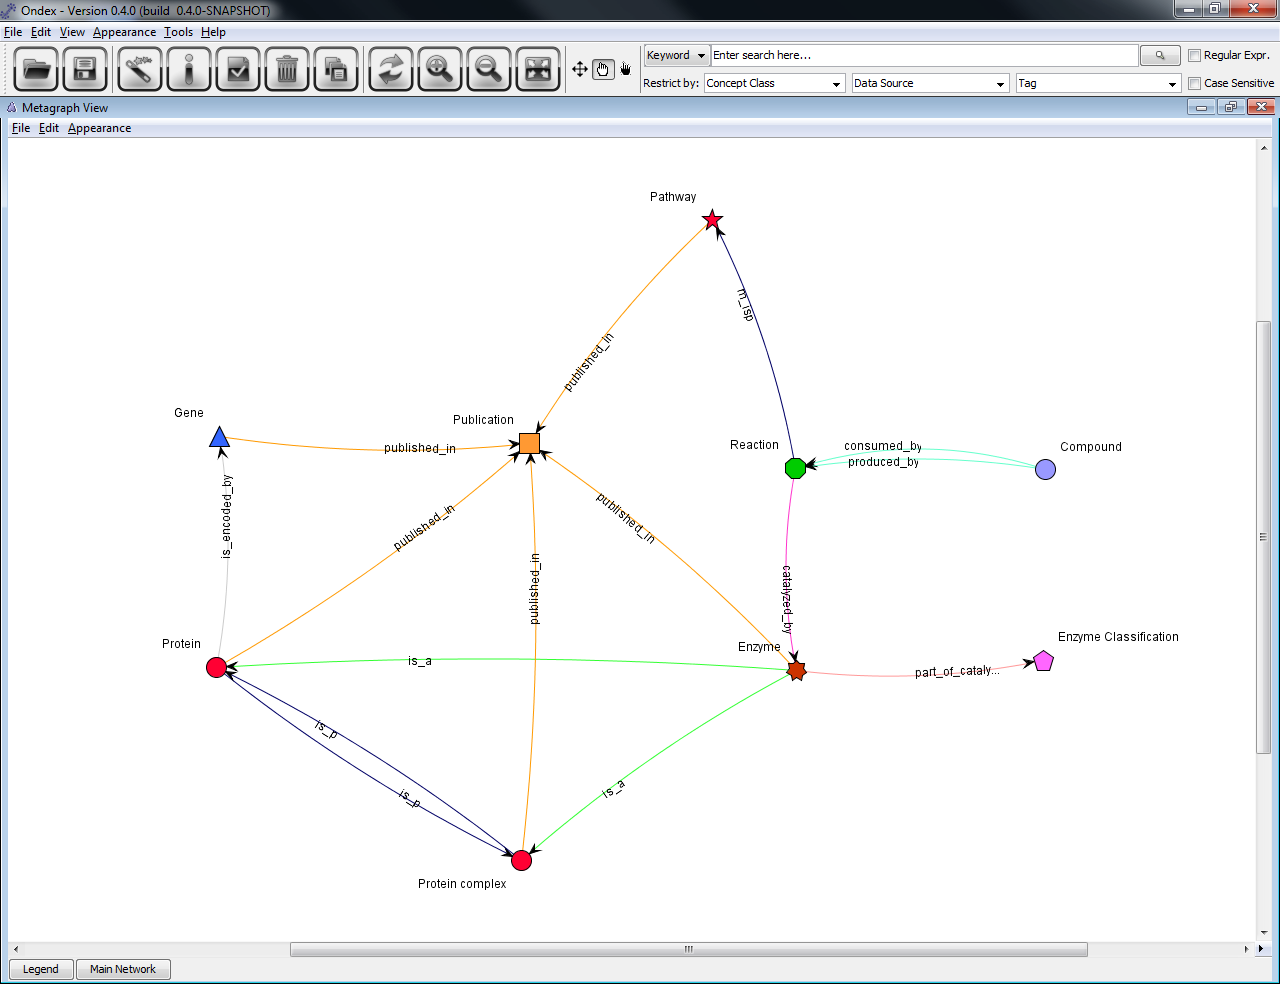
\includegraphics[scale=0.3]{images/Jun12/aracyc_rearranged_metagraph.png} 
\caption{Rearranged metagraph of AraCyc}
\label{fig:metagraph_rearranged}
\end{figure}
A protein is encoded by a gene (is\_encoded\_by).
A protein is part of a protein complex (is\_p).
An enzyme is a protein or a protein complex (is\_a).
An enzyme has a catalysing class EC (part\_of\_cataly...).
A compound is consumed by or produced by a reaction (consumed\_by, produced\_by).
A reaction is a member, is part of a pathway (m\_isp).
A reaction is catalysed by an enzyme (catalyzed\_by).
Finally, most concepts can be mentioned in publications (published\_in).

\exerciserule
\textbf{Exercise}
Right-click on nodes or edges in the metagraph displays the number of entities of that type in the network. 
It also gives users the opportunity to deselect ``Visible''. This will make concepts/relations of that type invisible in the main network. 
Nodes or edges in the metagraph for which all concepts/relations are invisible in the main network will appear in a paler colour.

\emph{Note:} Making concepts/relations invisible in the network will not delete them from the network altogether. 
If you wish to do so, use menu Edit -$>$ Delete Hidden Items. A window will pop up asking you for confirmation.

\exerciserule
\textbf{Exercise}
In the legend, clicking on colours/shapes will allow you to pick different colours/shapes for concept classes, 
data sources, relation types and evidence types (see 4 tabs in the legend window). 

For example, the concept class protein is of the same colour as the concept class pathway.
In order to make it more distinct, we can change its colour by clicking on the coloured rectangle (first column).
Figure \ref{fig:aracyc_click_colour} is obtained.
\begin{figure}[H]
\centering
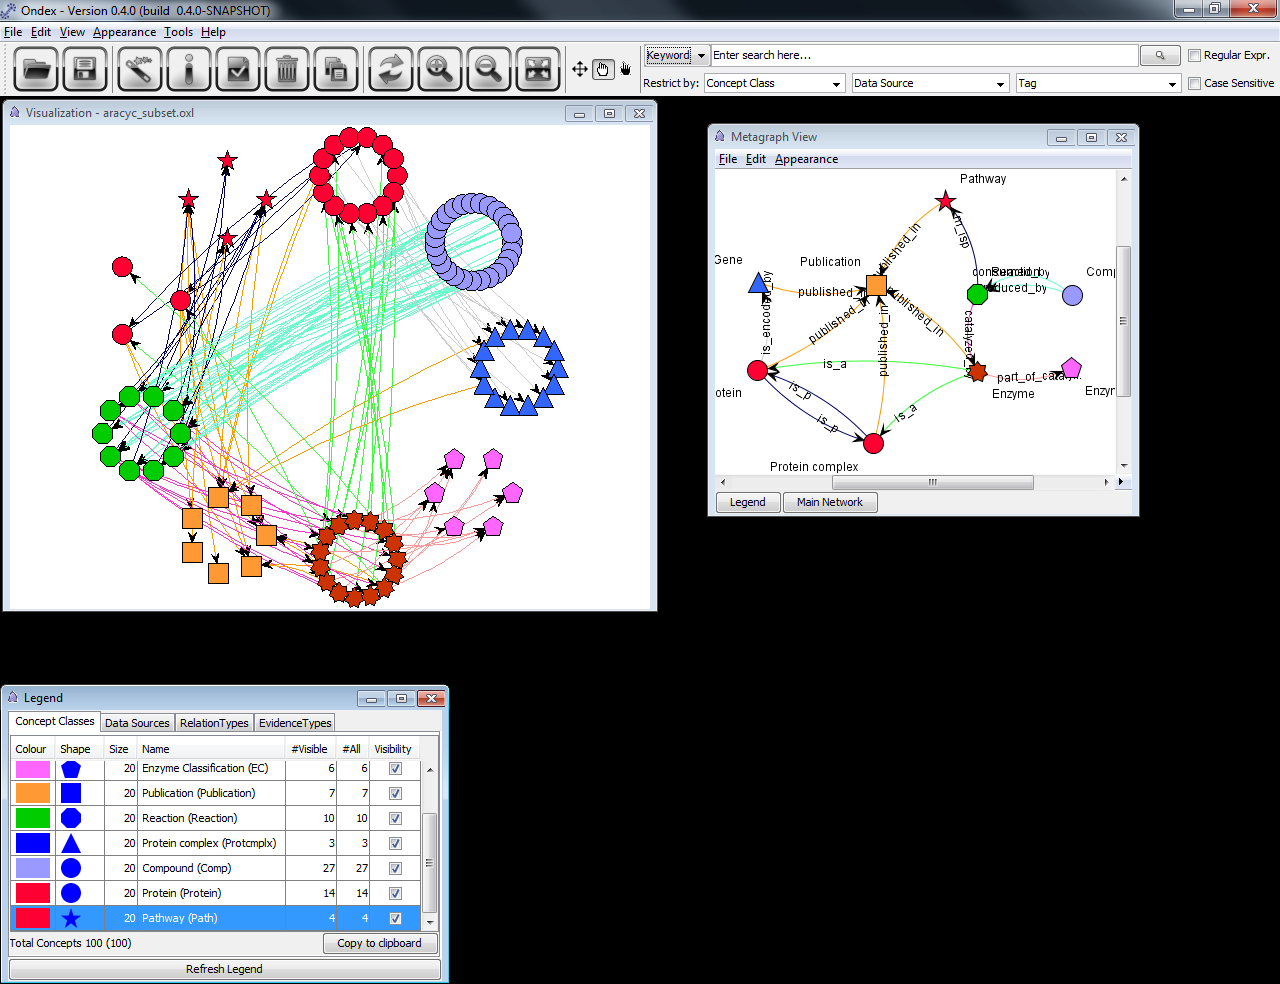
\includegraphics[scale=0.3]{images/Jun12/aracyc_colour_CC_from_legend.png} 
\caption{Click on a colour in the legend. A window pops open to change colours}
\label{fig:aracyc_click_colour}
\end{figure}

Clicking on the coloured rectangle pops open a ``Pick a colour'' window (see Figure \ref{fig:aracyc_pick}).
\begin{figure}[H]
\centering
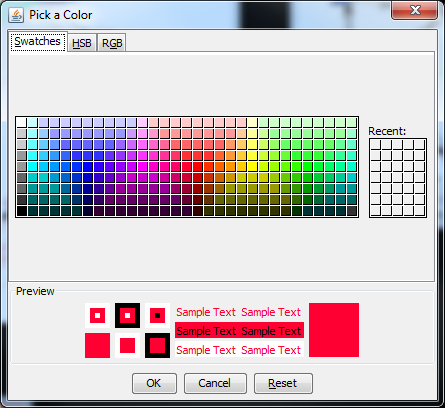
\includegraphics[scale=0.5]{images/Jun12/aracyc_pick_a_colour.png} 
\caption{Select a colour of your choice}
\label{fig:aracyc_pick}
\end{figure}

Select a colour, click on OK to obtain Figure \ref{fig:aracyc_changed_colour}.
\begin{figure}[H]
\centering
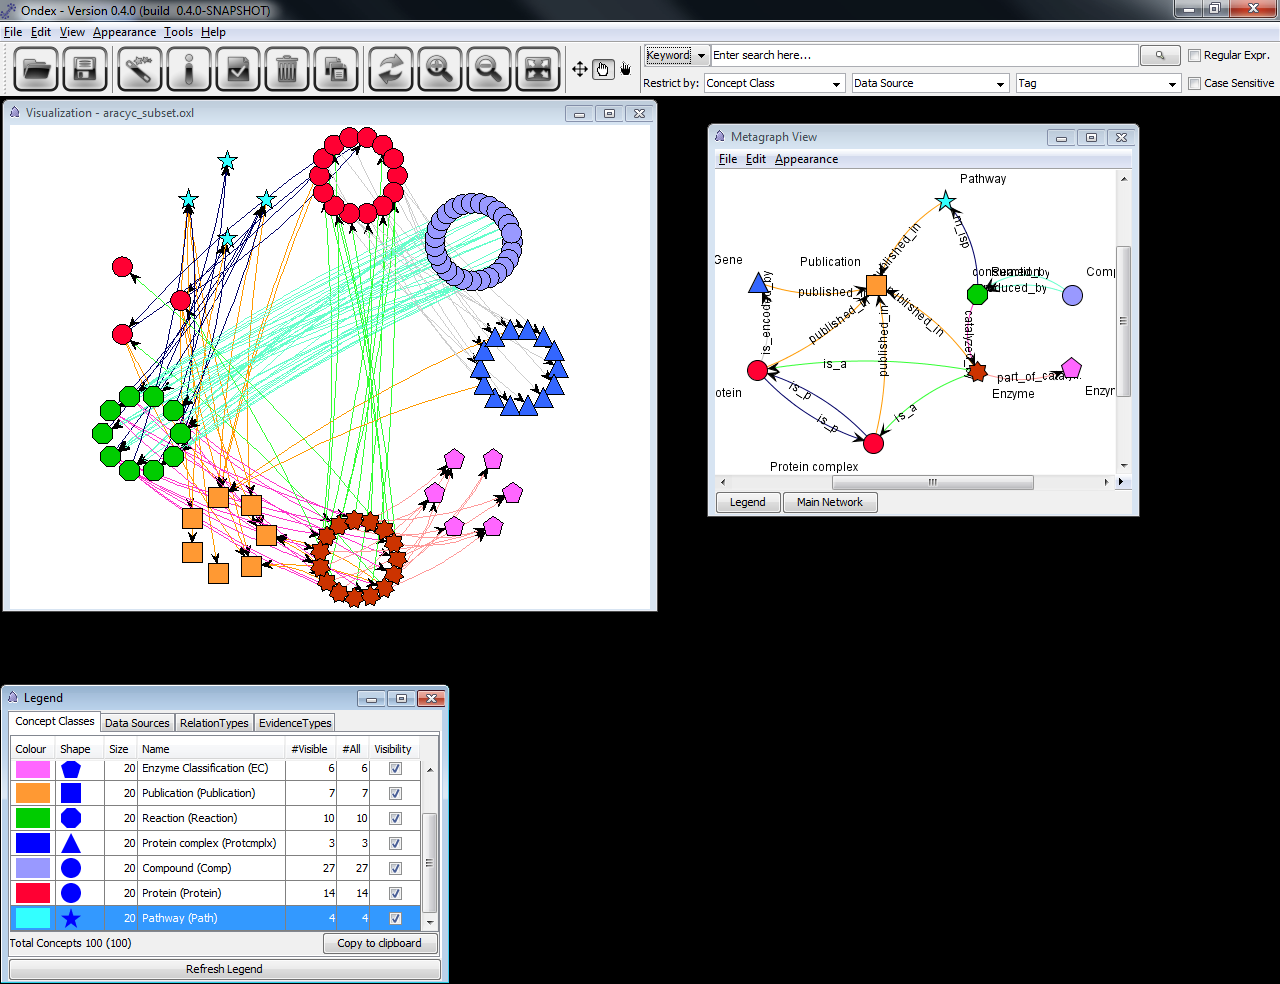
\includegraphics[scale=0.3]{images/Jun12/aracyc_colour_changed_from_legend.png} 
\caption{The colour of the concept class pathway has changed to turquoise}
\label{fig:aracyc_changed_colour}
\end{figure}

\exerciserule

The legend has four tabs: Concept Classes, Data Sources, Relation Types and Evidence Types. 
Figure \ref{fig:aracyc_legend_other_tabs} shows the Relation Types tab for this example.
Each tab displays the number of visible concepts/relations as well as the total number ({\it{i.e.}} including invisible items) in separate columns.
This window also allows you to select/deselect the check-boxes to make certain items visible/invisible in the visualisation window.
Furthermore, at the bottom of the legend window a total number is shown and a ``Copy to clipboard" button which enables users to copy/paste these numbers into other applications to keep track of them if needed.
\begin{figure}[H]
\centering
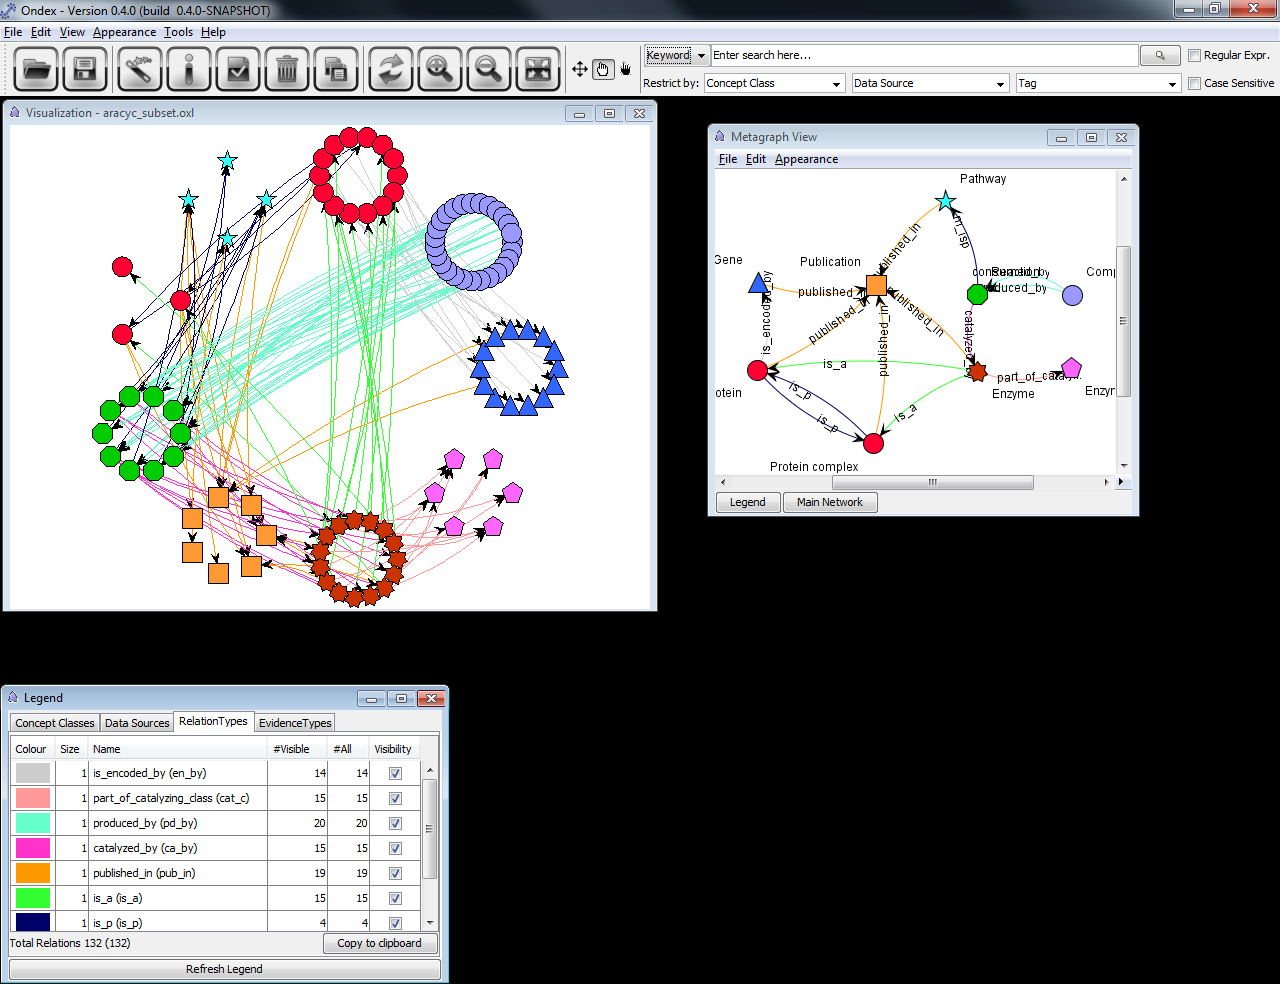
\includegraphics[scale=0.3]{images/Jun12/aracyc_legend_other_tabs.png} 
\caption{The Relation Types tab in the legend}
\label{fig:aracyc_legend_other_tabs}
\end{figure}

\emph{Advanced tip:} The experimental export plug-in "Graph Information Export" can be used when more thorough reports of the data are required for data integration purposes and can save a lot of time compared to manual inspection of graphs as it offers lists of accessions along with examples and percentages.
Such reports are particularly useful for setting the parameters of the accession based mapping method 
(see Sections \ref{sec:accmapping_examples} and \ref{sec:accmapping}) correctly.


%%%%%%%%%%%%%%%%%%%%%%%%%%%%%%%%%%%%%%%%%%%%%%%%%%%%%%%%%%%%%%%%%%%%%%%%%%%%%%%%%%%%%%%%%%%%%%%%%%%%%%%%%%%%%%%%%%%%%%%%%%%%%%%%%%%%%%%%%%%%%%%%%%%%%%%%%%
\section{Analysing Networks}
\label{sec:analysing}
If the main network is large and wasn't opened behind the metagraph, you can click on ``Main Network'' in the ``Metagraph View'' window or maximize the visualisation window that has been sitting in the bottom left-hand side corner all along.
Opening the visualisation window can take some time when there are a lot of concepts and relations to draw.
Two options are possible at this stage:
\begin{enumerate}
\item If your computer is fast or you are patient, you can open the main network as described above
\item Otherwise you can use filters (under Tools menu) or a search (search bar, top-right corner) to extract a smaller sub-network.
If the data contains ``tags'' (predefined subsets of the data) then using the Tag Filter is another possibility.
\end{enumerate}

%%%%%%%%%%%%%%%%%%%%%%%%%%%%%%%%%%%%%%%%%%%%%%%%%%%%%%%%%%%%%%%%%%%%%%%%%%%%%
\subsection{Filtering}
\label{sec:filtering}

For example here, rather than looking at the whole subset of AraCyc in Figure \ref{fig:complete_subset_aracyc}, 
let us select a single pathway to display.

\begin{figure}[H]
\centering
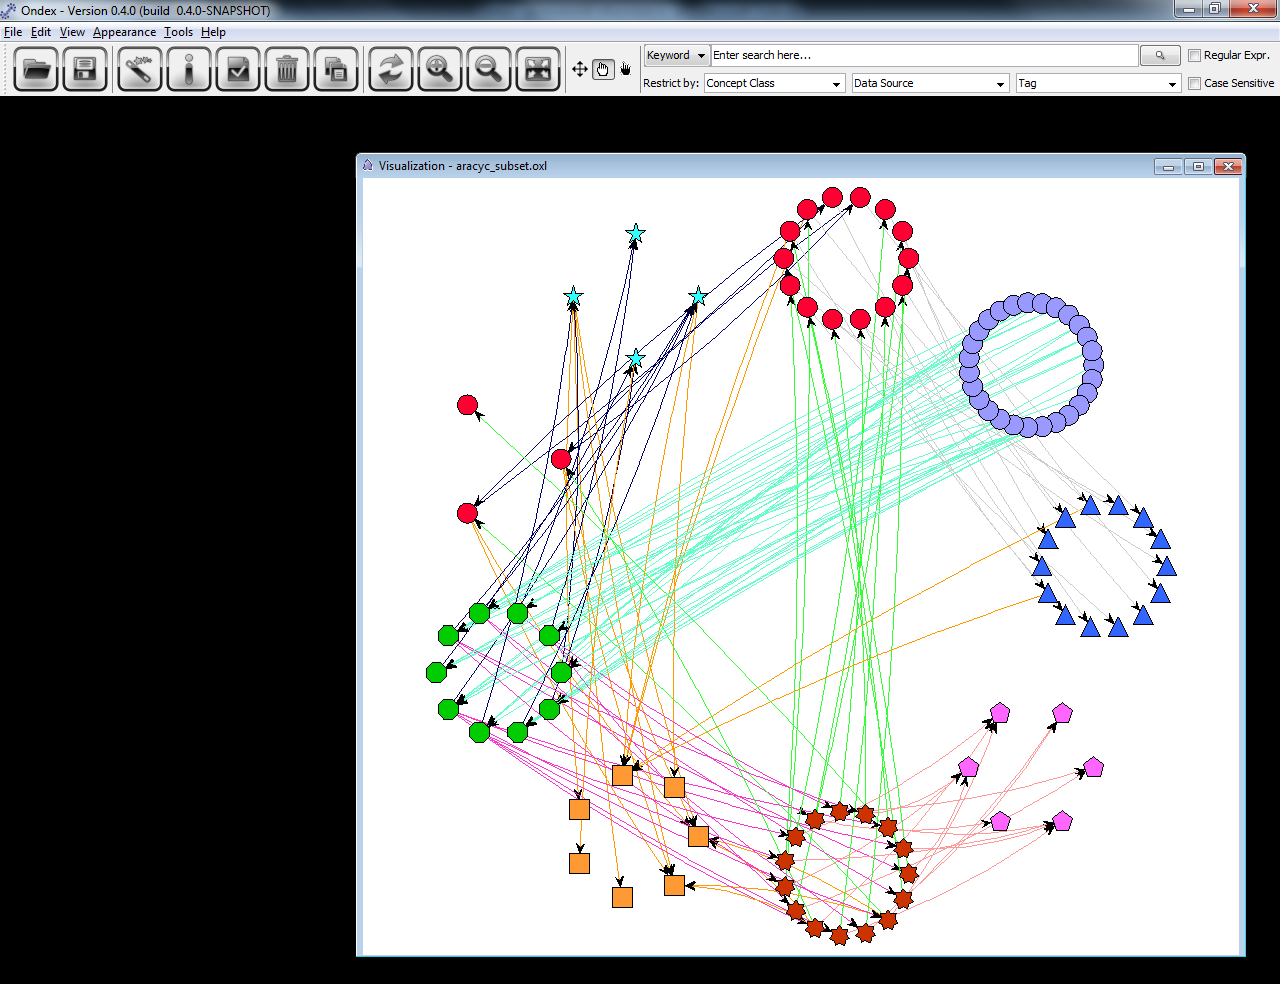
\includegraphics[scale=0.3]{images/Jun12/aracyc_circular_subset.png} 
\caption{Subset of AraCyc drawn with the circular (default) layout}
\label{fig:complete_subset_aracyc}
\end{figure}

In order to do so, select the Tag Filter under menu Tools -$>$ Filters.
This filter is fully explained in the ``F1 help'' documentation of Ondex.
It offers the possibility of combining different tags.
For now, we will simply filter down the network to a single pathway.
Let us select GDP-L-fucose biosynthesis II as shown in Figure \ref{fig:aracyc_pick_tag}
(click on the view tag cell and select GDP-L-fucose biosynthe... from the list of possible tags).

\begin{figure}[H]
\centering
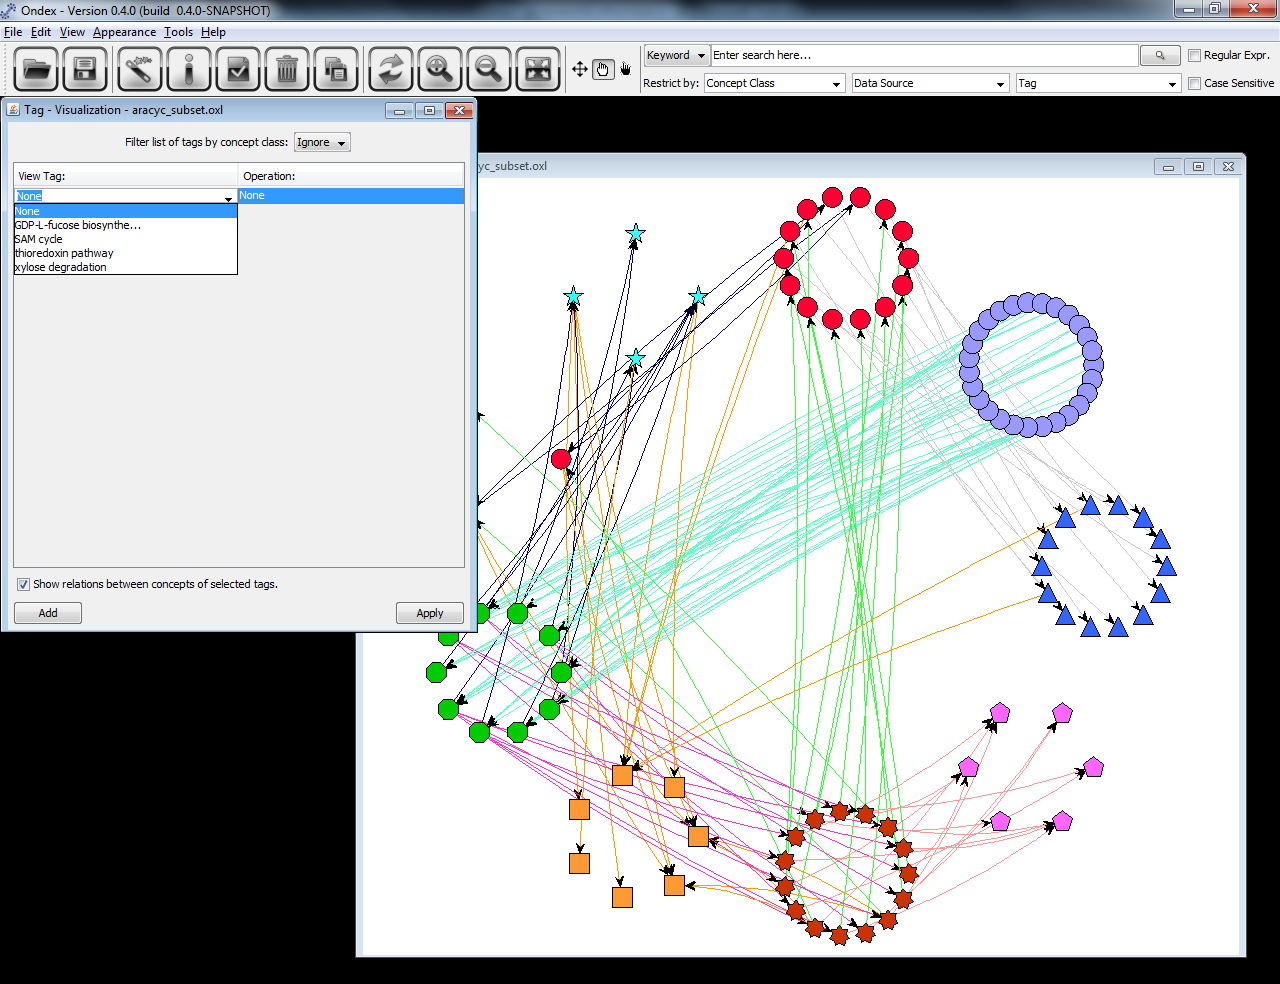
\includegraphics[scale=0.3]{images/Jun12/aracyc_pick_tag.png} 
\caption{Pick a tag from the drop-down list}
\label{fig:aracyc_pick_tag}
\end{figure}

Figure \ref{fig:aracyc_gdp_fucose_II} shows the resulting network.
\begin{figure}[H]
\centering
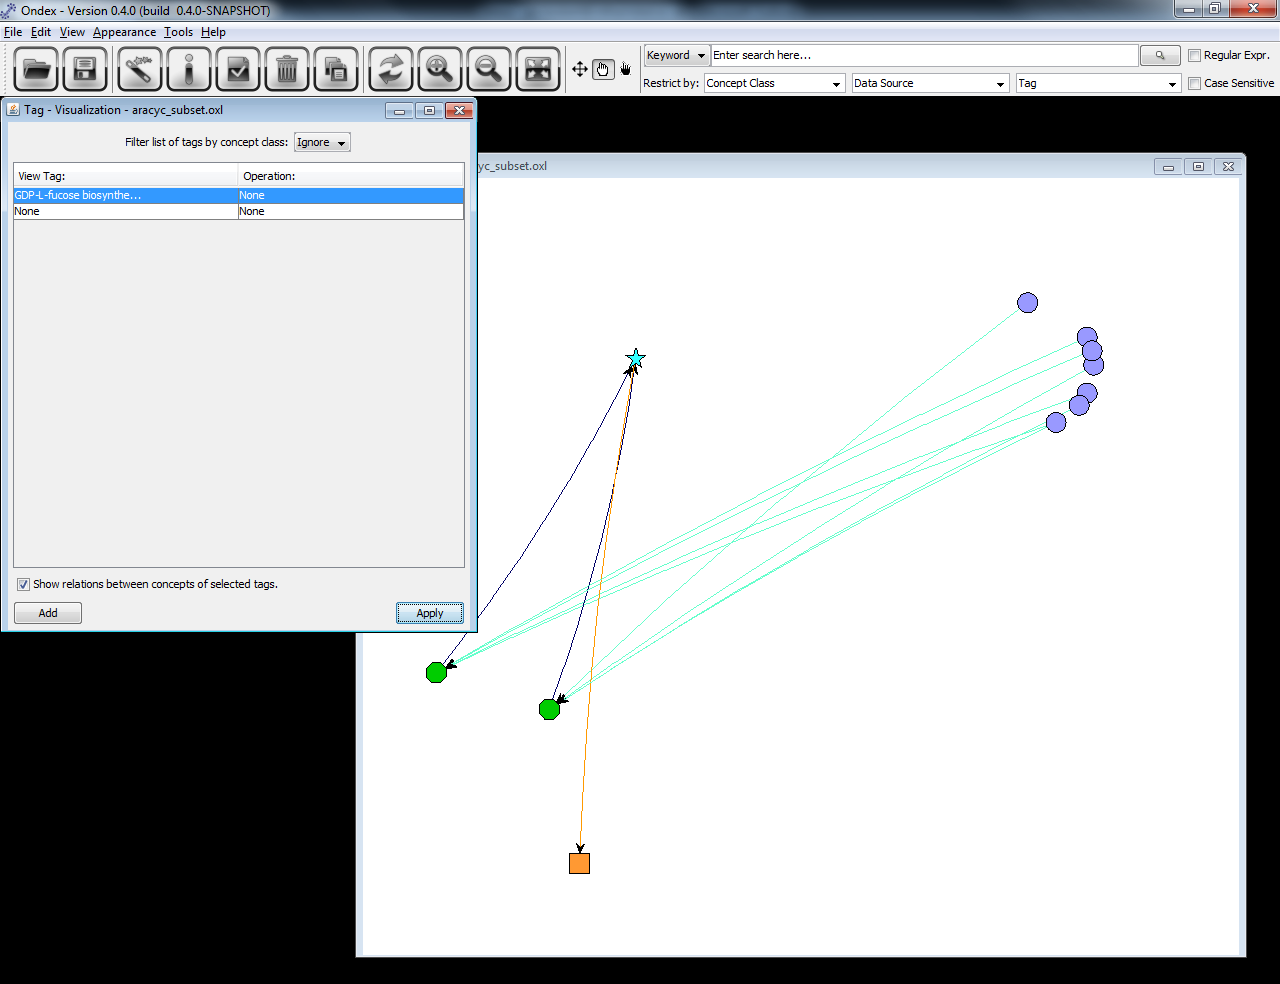
\includegraphics[scale=0.3]{images/Jun12/aracyc_gdp_fucose_II.png} 
\caption{The GDP-L-fucose biosynthesis II pathway from the AraCyc database}
\label{fig:aracyc_gdp_fucose_II}
\end{figure}

We can use Appearance -$>$ Layouts -$>$ More -$>$ Hierarchical for Ondex to organise the concepts hierarchically (see Figure \ref{fig:aracyc_gdp_fucose_hierarchical}).
\begin{figure}[H]
\centering
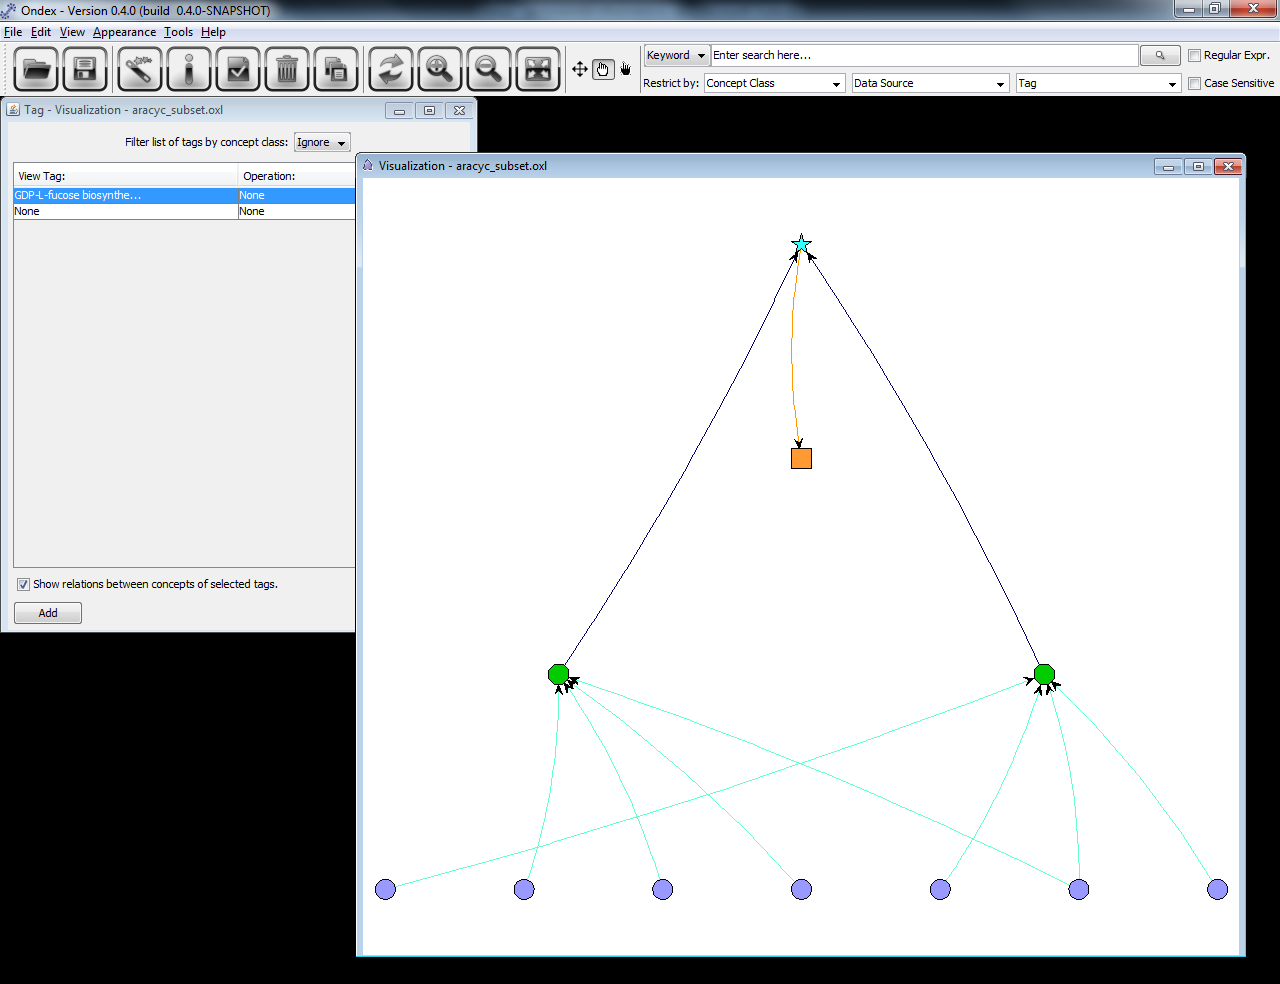
\includegraphics[scale=0.3]{images/Jun12/aracyc_gdp_fucose_hierarchical.png} 
\caption{Hierarchical layout of the GDP-L-fucose biosynthesis II pathway from the AraCyc database}
\label{fig:aracyc_gdp_fucose_hierarchical}
\end{figure}

You can then select a concept, for example, the pathway itself (click on it, it will become yellow).
Then you can click on the ``i'' icon (a tool-tip shows when you mouse over the icon) to see information about the selected pathway, as shown in Figure \ref{fig:aracyc_gdp_fucose_iteminfo}. \emph{Note:} You can ignore the ``Taxonomy lookup'' by clicking on the given option ``No, don't ask again''.


The item information gives a link to the AraCyc website at the very bottom of the window under section ``Accessions''.
Clicking on this link opens a web browser as shown in \ref{fig:aracyc_info_website}.
\begin{figure}[H]
\centering
\subfigure[Item Information icon launches an information window]{
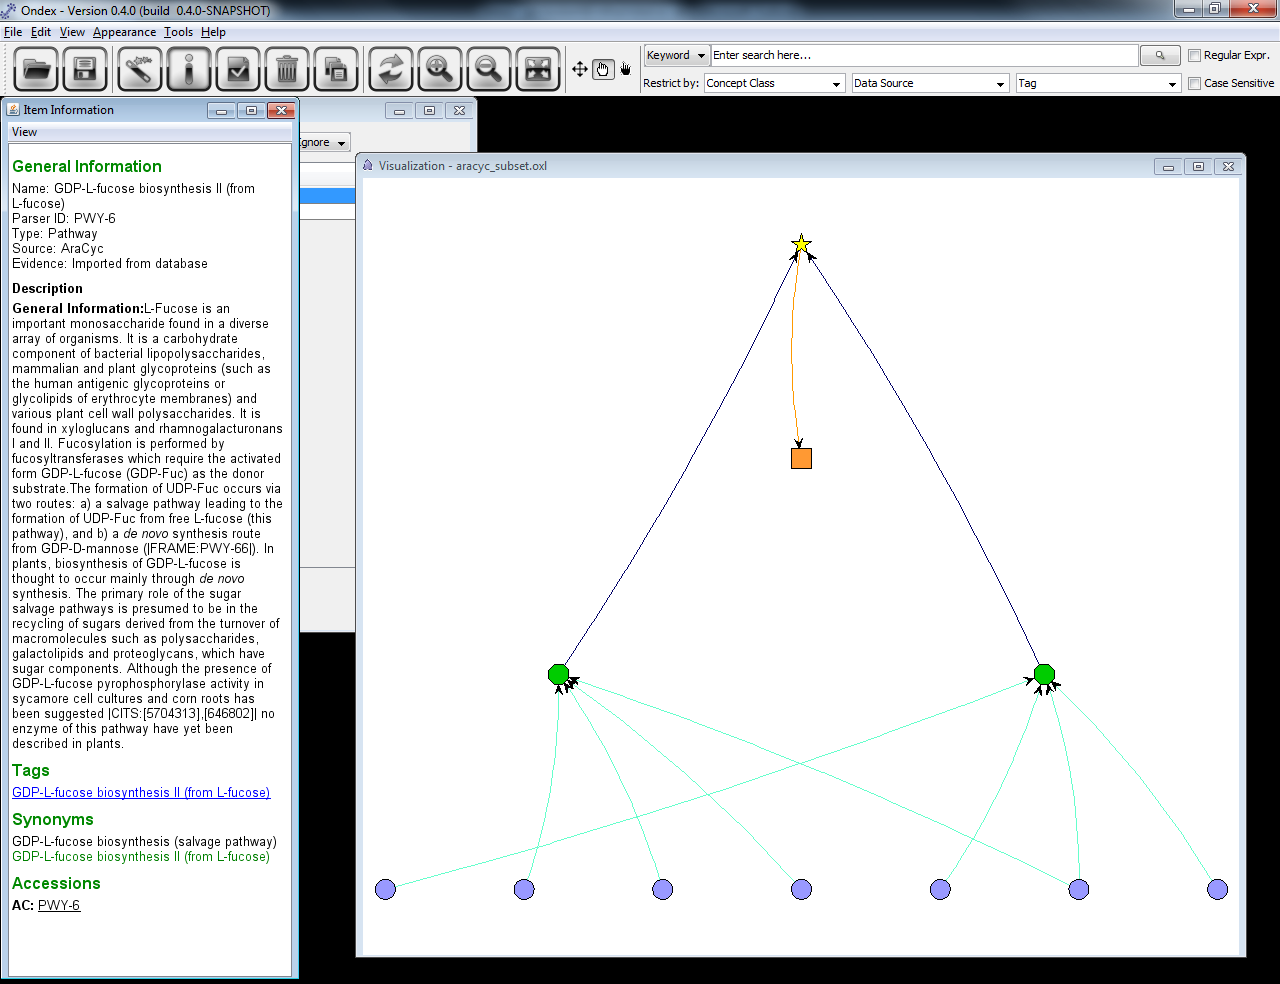
\includegraphics[scale=0.3]{images/Jun12/aracyc_gdp_fucose_iteminfo.png} 
\label{fig:aracyc_gdp_fucose_iteminfo}
}
\subfigure[The Aracyc website showing the selected pathway]{
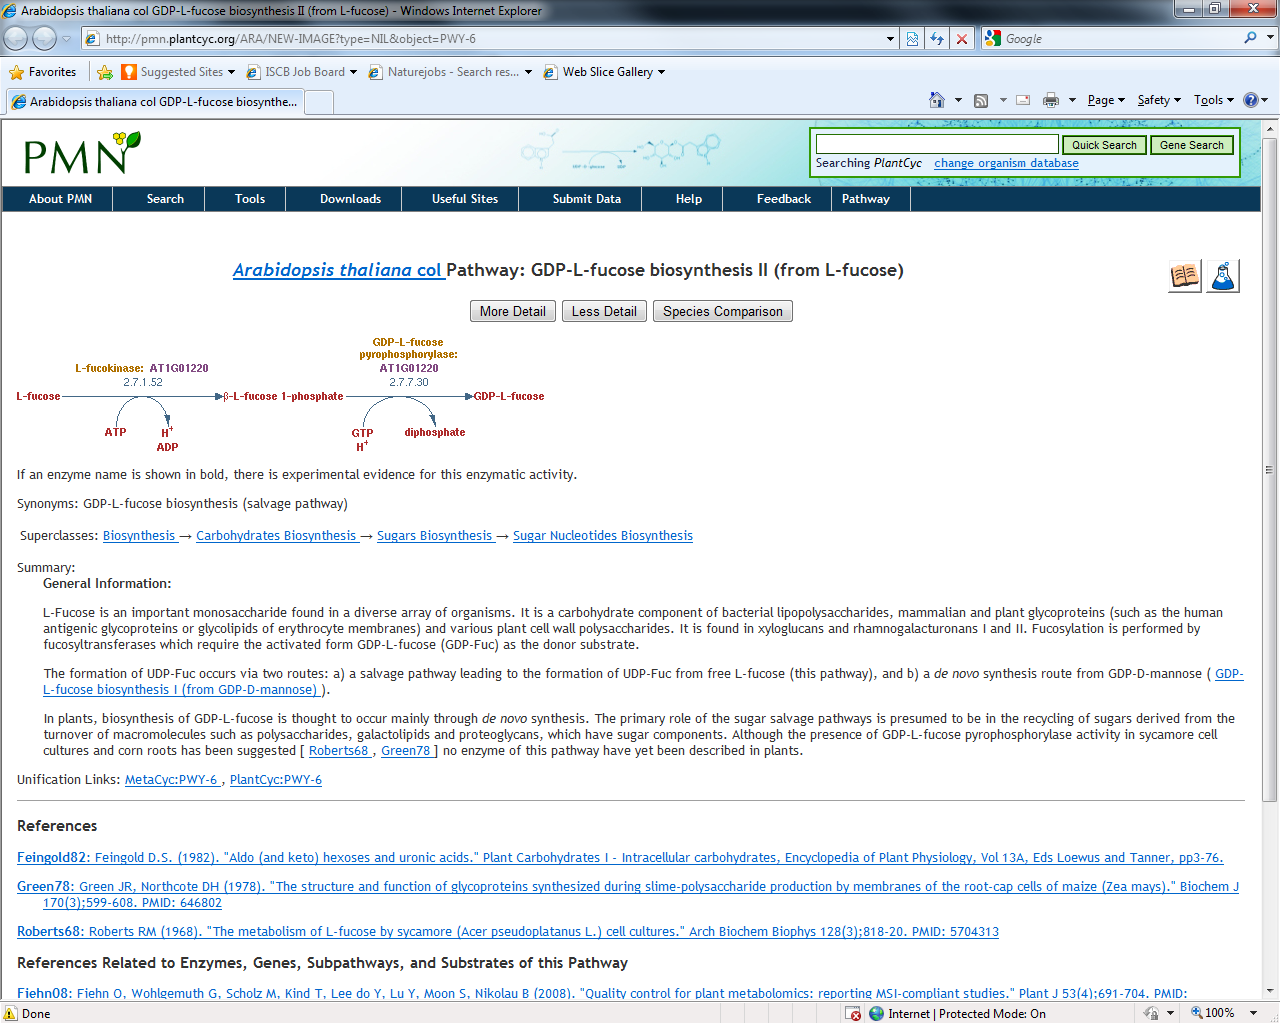
\includegraphics[scale=0.3]{images/Jun12/aracyc_gdp_fucose_webpage.png} 
\label{fig:aracyc_gdp_fucose_webpage}
}
\label{fig:aracyc_info_website}
\caption[optional]{Item information and its links to websites}
\end{figure}

\vspace{0.5cm}
\exerciserule
\textbf{Exercise }
Study the reaction shown on the website and try to understand how it is represented in Ondex.

\emph{Help:} The first thing you might want to do is use the menu Appearance -$>$ Labels to add concept and relation labels 
on the network so you know what is what without needing the ``Item Information'' window. Use
Appearance -$>$ Labels -$>$ Both to show labels of concepts and relations.

\emph{Help:} To move concepts around, you can either pick them (in picking mode - ``white hand'' icon before search bar in the tool-bar or menu Edit -$>$ Mouse mode -$>$ Picking) and move them one by one.
You may also press shift to select a few concepts with the left mouse button and
using the left mouse button again you can drag these group of concepts around.

Figure \ref{fig:aracyc_gdp_fucose_sorted} shows what can be obtained by following this process. 
\emph{Note:} the ``Metagraph View'' window is not shown on this screenshot.
The reactions previously shown on the website have been reconstituted. 
Here, the compound that is a product of the first reaction and a substrate of the second has been selected and is automatically shown in the ``Item Information'' window.\\ 
\emph{Note:} SMILES stand for ``simplified molecular input line entry specification''.\\
\emph{Note:} If you have closed the Legend (previously launched from the metagraph view window), you may launch it again using View -$>$ Legend to check how many compounds are currently displayed.
\begin{figure}[H]
\centering
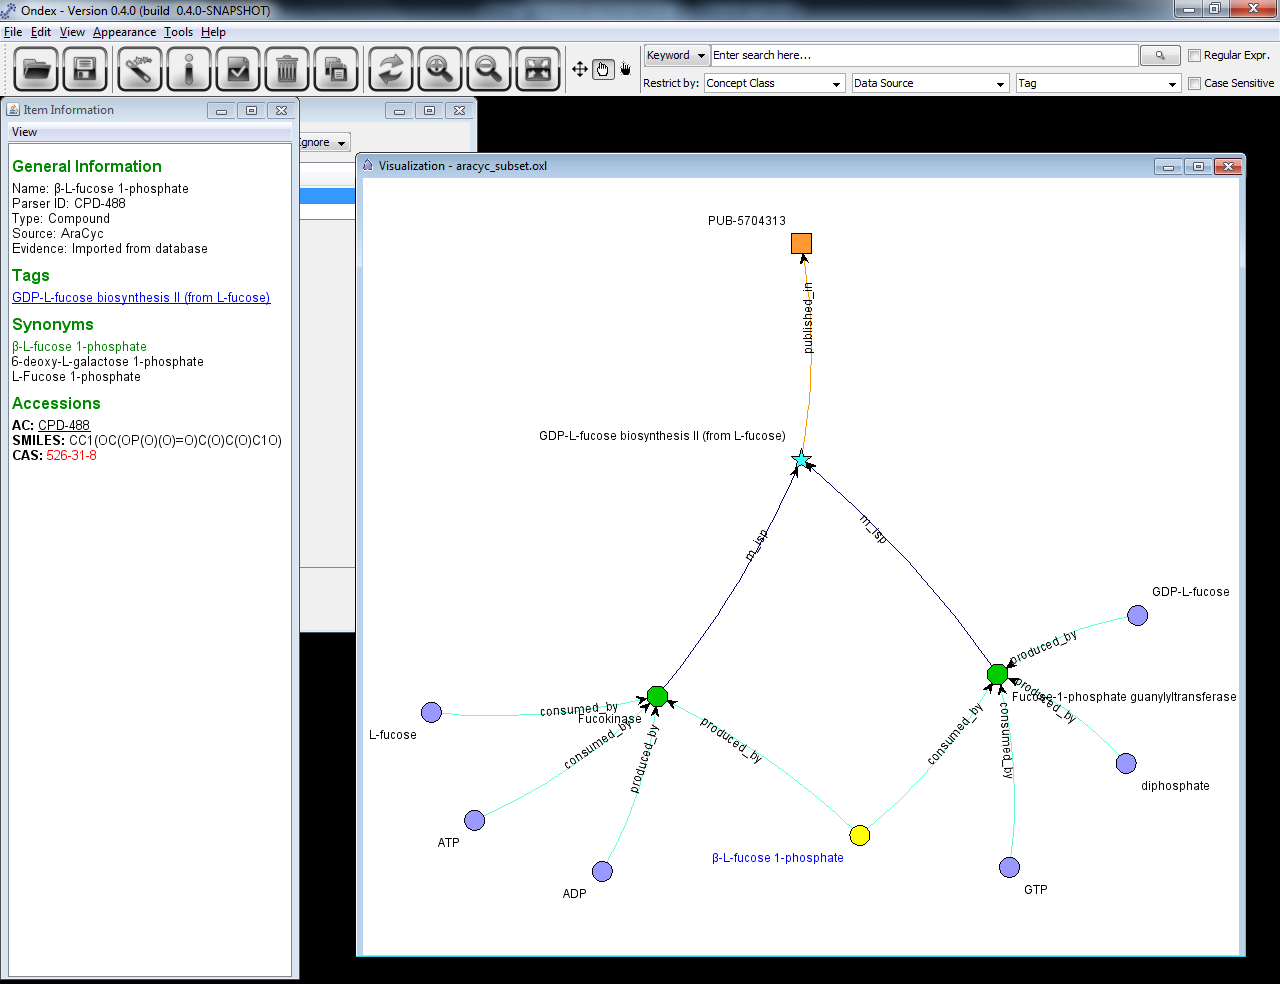
\includegraphics[scale=0.3]{images/Jun12/aracyc_gdp_fucose_sorted.png} 
\caption{The GDP-L-fucose biosynthesis II pathway as shown in Figure \ref{fig:aracyc_gdp_fucose_webpage} layout in Ondex}
\label{fig:aracyc_gdp_fucose_sorted}
\end{figure}
\exerciserule

Other filters and annotators (as well as layouts) are available and documented in Ondex.
Users can press F1 to access this documentation at any time.
They can also place their mouse over tool-tips for a short description to pop up,
or click on the blue question mark icon for the documentation window to open.
In Tutorial\_files/Annotators\_and\_Filters/readme\_annotators\_filters.txt explains which file (within that directory) 
is used for each example in the documentation's screenshots (to allow users to play with the data themselves).

%%%%%%%%%%%%%%%%%%%%%%%%%%%%%%%%%%%%%%%%%%%%%%%%%%%%%%%%%%%%%%%%%%%%%%%%%%%%%
\subsection{Searching}
\label{sec:search}
Ondex includes a Search feature (see Figure \ref{fig:vis_search_bar}), which enables you to quickly find concepts in the network containing a given keyword or by chemical similarity to a given SMILES or InChI qualifier.
\begin{figure}[H]
\centering
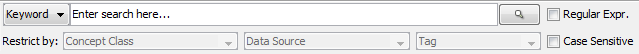
\includegraphics[scale=0.6]{images/Jun12/search_bar.png} 
\caption{The Ondex search bar}
\label{fig:vis_search_bar}
\end{figure}

For example, searching for keyword fucose in our current graph will give use the results shown in Figure \ref{fig:search_results}
\begin{figure}[H]
\centering
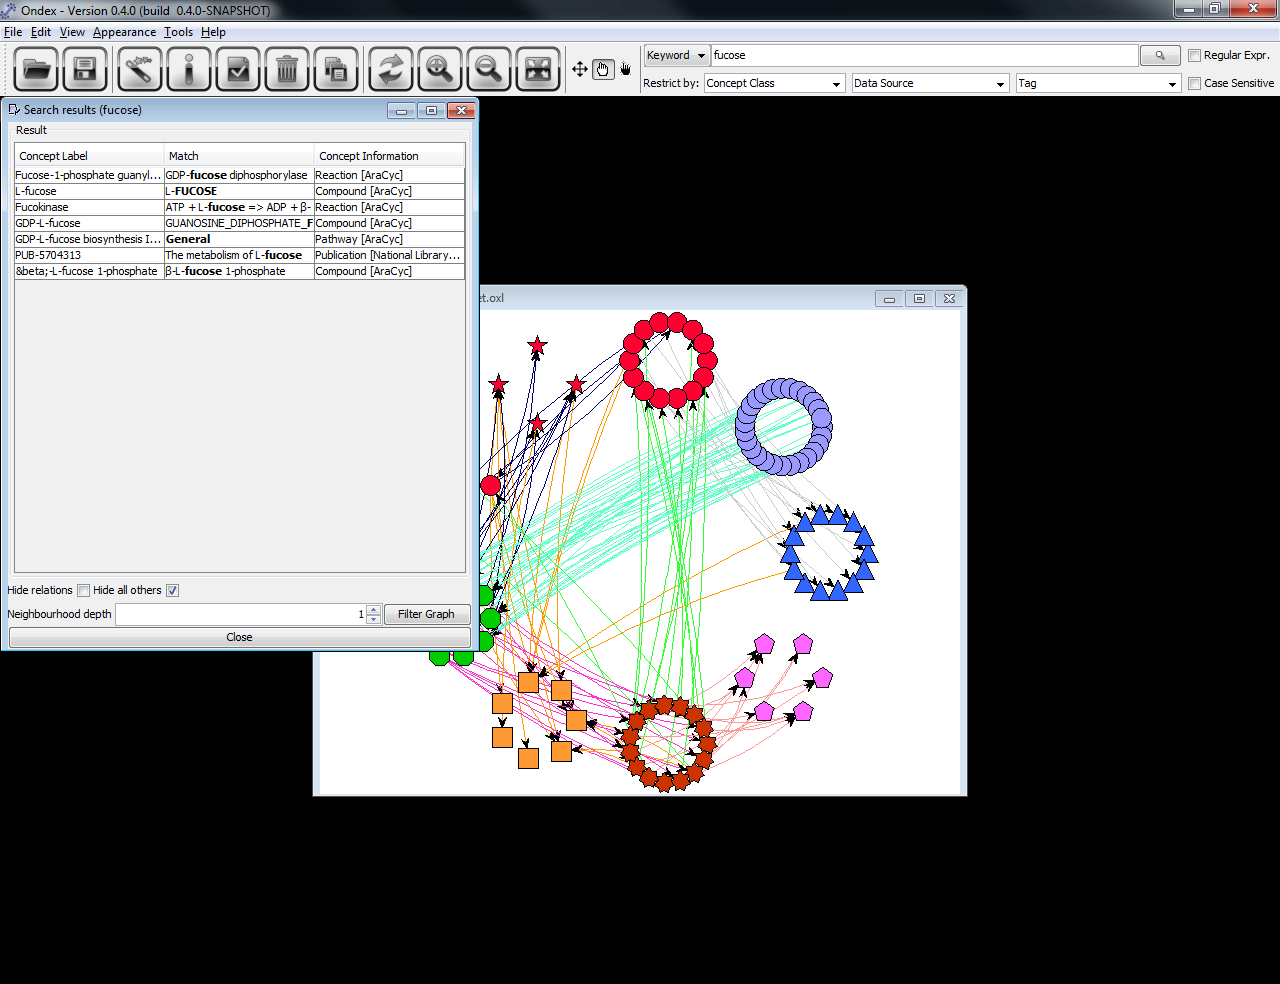
\includegraphics[scale=0.3]{images/Jun12/aracyc_search_fucose.png} 
\caption{Search results for ``fucose'' in Aracyc}
\label{fig:search_results}
\end{figure}

If you select (single click) one item in the search results, you will need to single click on the icon ``Zoom In'' in order for Ondex to zoom in and center on this particular concept. 
You can then use the mouse scroll wheel to zoom even closer to the concept.
If you select several items (using the Control key) in the search results, Ondex will automatically zoom in to show all those items as close as possible.

\vspace{0.5cm}\textbf{Configuring an Ondex Search }
\begin{itemize}
\item At the end of the tool-bar, there are 2 options that can be configured for keyword based search. 
If you select ``Regular Expression'', you may enter a Java regular expression. An example would be: AT$\backslash$dG.
It will match ``AT'' followed by any digit and ``G''. For more information on regular expressions in Java, please visit \url{http://docs.oracle.com/javase/tutorial/essential/regex/}.
If you select ``Case Sensitive'', the search will be sensitive to lower/upper case of each character.
\item Under the search box, there are 3 drop-down lists which allow users to restrict their search (by Concept Class, Data Source or Tag).
An example is provided in the next section's exercise.
\end{itemize}

%%%%%%%%%%%%%%%%%%%%%%%%%%%%%%%%%%%%%%%%%%%%%%%%%%%%%%%%%%%%%%%%%%%%%%%%%%%%%
\subsection{Right-clicking}
\label{sec:right-clicking}
Right-clicking on one or a selection of concepts/relations also offers users the possibility to narrow down the graph to what they are interested in.
Close all the windows you have opened in Ondex (View -$>$ Windows -$>$ Close All).

\begin{itemize}
\item Go to File -$>$ Open  (or click on the first button in the icon bar)
\item You should see an Open File Dialog
\item Open the Tutorial\_files/Main\_part folder, select poplar\_exercise1.oxl and click on open
\end{itemize}

This graph results from a data integration (see Chapter \ref{cha:integration}) pipeline using information from JGI,
UniProtKB, TAIR, Gramene, Gene Ontology (GO), GOA (GO Annotations), TraitOnt, PlantOnt, Medline, AraCyc, PoplarCyc and Pfam
which aims to identify genes controlling biomass production in willow.
The willow genome is not yet sequenced. Poplar is the first tree with fully sequenced genome but
not much is known yet about the function of poplar genes.
This study (see Chapter \ref{cha:qtl}) uses a comparative genomics approach to compare poplar to {\it{Arabidopsis}} and rice.

The metagraph shows a lot of different concept classes and relation types,
including ``Molecular Function'', ``Biological Process'' and ``Cellular Compartment'' - the 3 GO categories (see Figure \ref{fig:vis_poplar_metagraph}).
\begin{figure}[H]
\centering
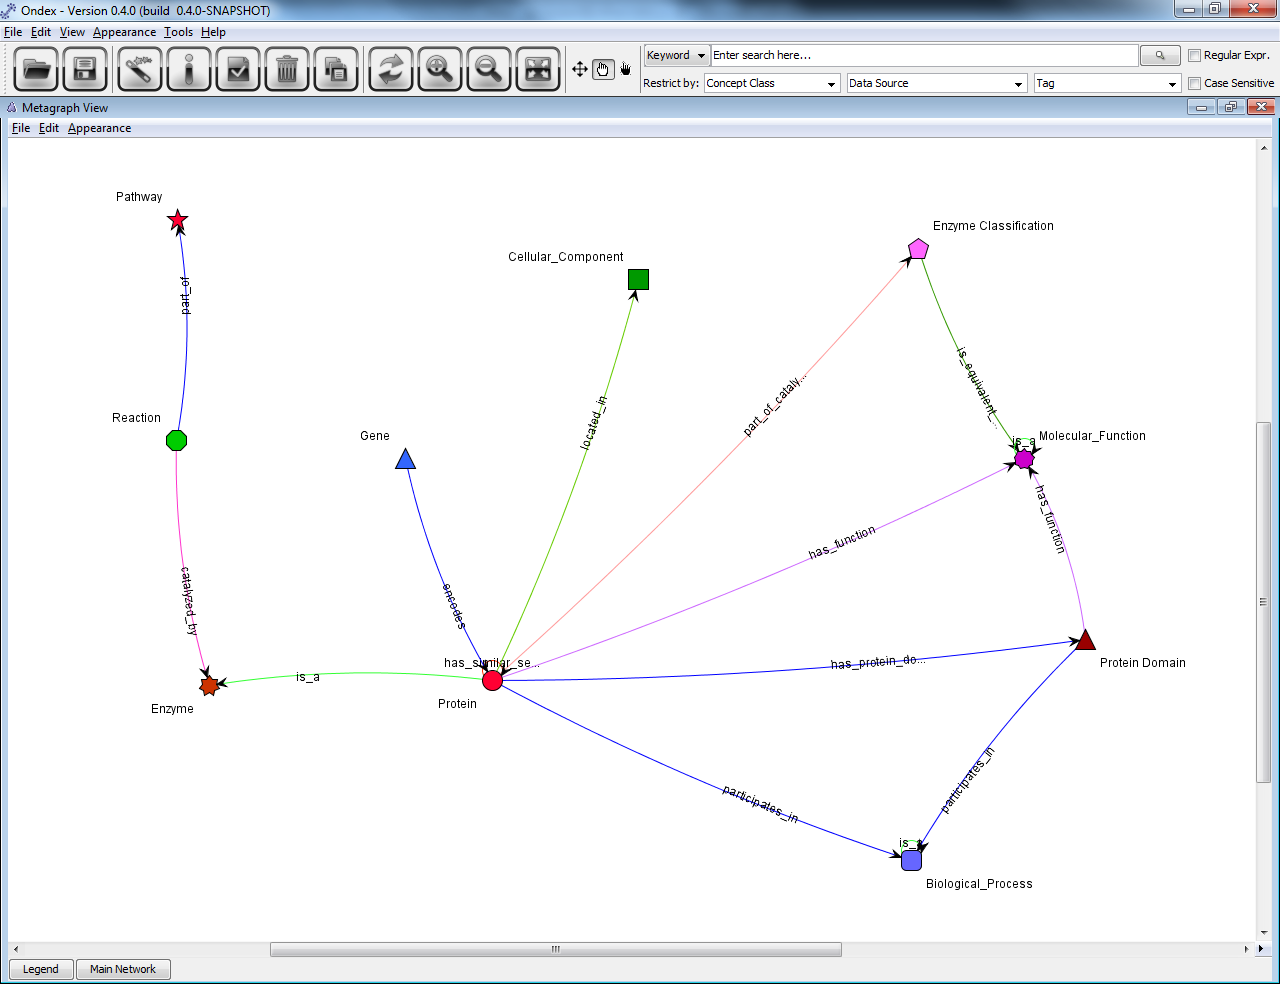
\includegraphics[scale=0.3]{images/Jun12/poplar_ex1_metagraph.png} 
\caption{Metagraph - poplar\_exercise1.oxl}
\label{fig:vis_poplar_metagraph}
\end{figure}

\exerciserule
\textbf{Exercise}
In this exercise, we will look at a particular poplar gene (the only one in this subset). 
As it is lacking functional annotation, we wish to study the poplar protein it encodes, its homologous proteins 
and the GO terms they have been associated with. We will also investigate whether data integration has allowed linking this poplar protein to other kinds of information.
Use the search bar and a combination of right-clicks to get to Figure \ref{fig:poplar_result_exercise1} where only these concepts are visible on the graph.
\begin{figure}[H]
\centering
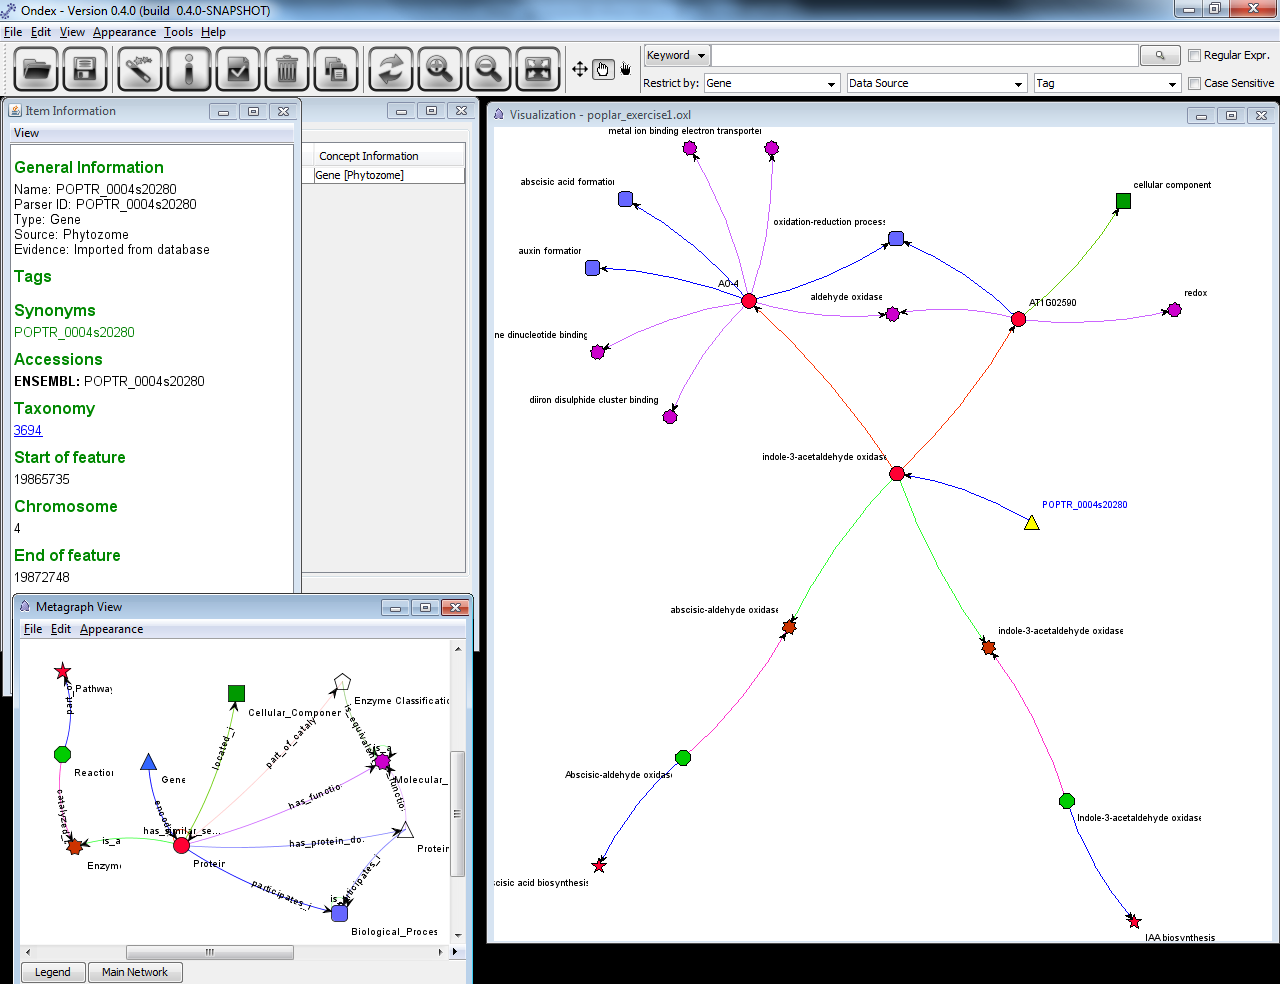
\includegraphics[scale=0.3]{images/Jun12/poplar_result_exercise1.png} 
\caption{Visualisation window (and part of metagraph) at the end of the exercise}
\label{fig:poplar_result_exercise1}
\end{figure}

\emph{Help:} 
\begin{itemize}
\item Clear the search bar, restrict the search to Concept Class Gene and hit enter. You should obtain only one result (because there was only one gene in this particular subset).
\item In the search results, select a neighbourhood depth of 1 and click on ``Filter Graph''.
\item Click on Main Network (from the metagraph or from the minimized window), you should see the gene you had searched for and the protein encoded by that gene.
\item Click on Appearance -$>$ Labels -$>$ Concepts to show concept labels.
\end{itemize}

We are now interested in looking at homologous proteins which might be annotated with GO terms.
\begin{itemize}
\item Right-click on the protein and select Show -$>$ Immediate Neighbours by Concept Class -$>$ Protein(2:2). (There are two of them and both are invisible at the moment.)
\item Select the homologous proteins and check their item information using the ``i'' icon or View -$>$ Item Info. You will find one is from rice and one {\it{Arabidopsis}}.
\item Select the two homologous proteins (click on one, it becomes yellow, press shift and select the second one)
\item Right-click and select Show -$>$ Immediate Neighbourhood and observe the 3 categories of GO terms one by one, see how many are shared by the two orthologous proteins.
\end{itemize}

Now let's investigate whether data integration has allowed linking our poplar protein to other kinds of information.
\begin{itemize}
\item From our poplar protein, select Show -$>$ Immediate Neighbourhood. Protein domains and two enzymes show.
\item From the enzymes, select Show -$>$ Immediate Neighbourhood. Two reactions get displayed.
\item From the reactions, select Show -$>$ Immediate Neighbours by Concept Class -$>$ Pathway (2:2). Two pathways show.
\item You may study the protein domains and decide to show their relations to visible concepts on the graph (right-click Show -$>$ Relations to other Visible Concepts).
To get to Figure \ref{fig:poplar_result_exercise1}, you will need to hide them. 
To do so, you may select one protein domain and select Hide -$>$ Same Concept Class.
\end{itemize}

%%%%%%%%%%%%%%%%%%%%%%%%%%%%%%%%%%%%%%%%%%%%%%%%%%%%%%%%%%%%%%%%%%%%%%%%%%%%%
\subsection{Annotating}
\label{sec:annotating}
Once a graph is filtered down to a region of interest, annotators (Tools -$>$ Annotators) allow you to scale your concepts/relations,
change their shapes and colours or display numerical data as charts based on the attributes they hold.
We will work on a data integration problem described in Section \ref{cha:qtl} and analyse the results using a few annotators. Other application cases also show case various annotators.

This example allows you to practice analysing networks in Ondex using a combination of the tools available.
Firstly, given a candidate gene (the only one in the graph) we wish to study its annotations and their GO hierarchy.
We also wish to annotate the molecular functions based on their information content.
To do so:
\begin{itemize}
\item Load the Tutorial\_files/Main\_part/poplar\_exercise1.oxl dataset
\item Select the only gene in the graph (or search for it as we did in the previous exercise).
\item Run the shortest path filter. The results are shown on Figure \ref{fig:poplar_result_shortestpath}. 
\begin{figure}[H]
\centering
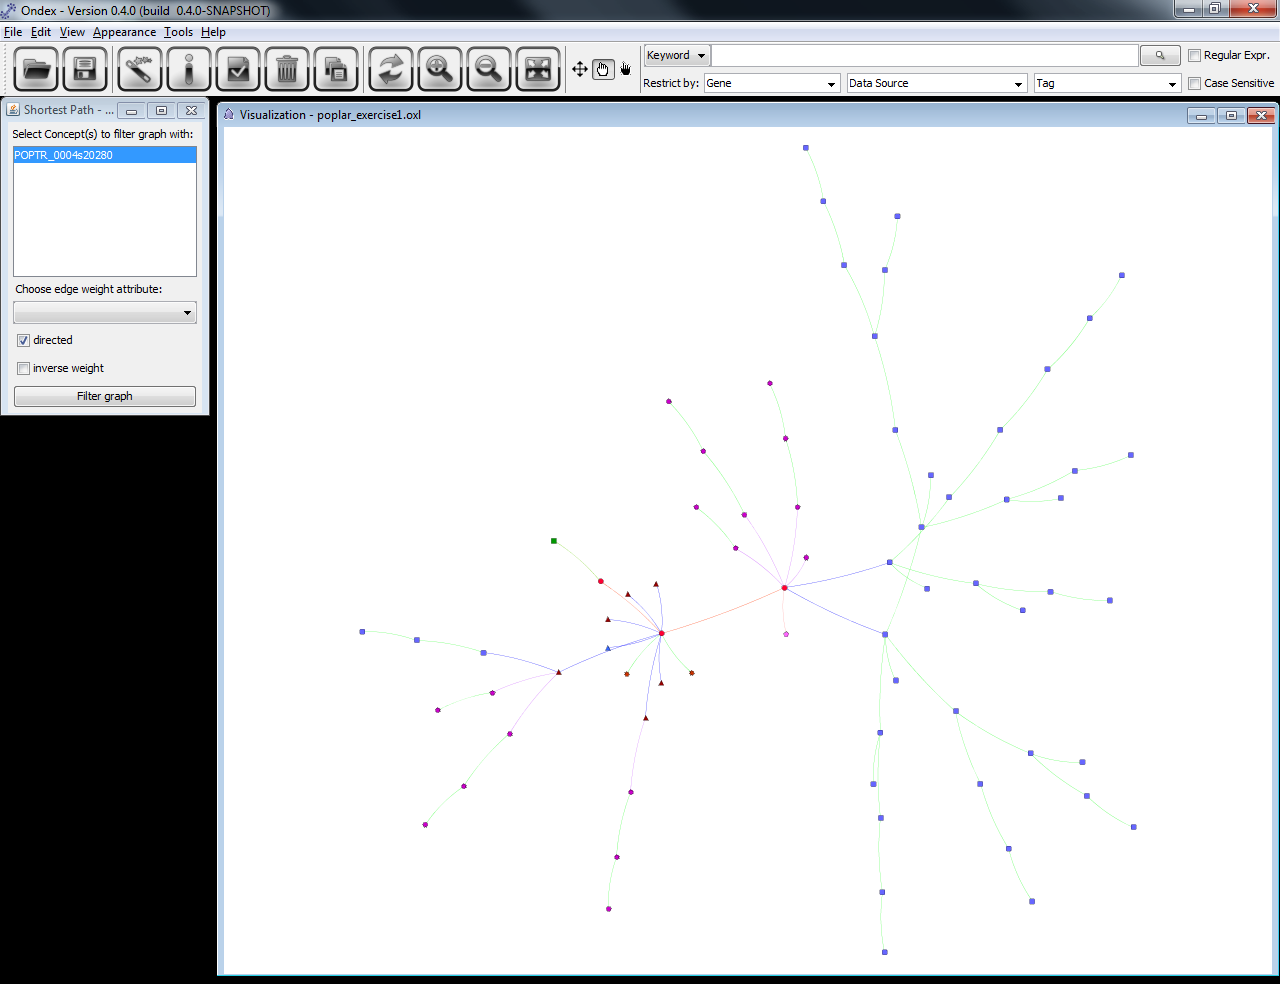
\includegraphics[scale=0.3]{images/Jun12/poplar_result_ex2_shortestpath.png} 
\caption{Screen-shot after applying the shortest path filter}
\label{fig:poplar_result_shortestpath}
\end{figure}

\emph{Help:}
	\begin{itemize}
	\item Tools -$>$ Filters -$>$ More -$>$ Shortest Paths -$>$ Shortest Path
	\item Select the gene (POPTR\_0004s20280)
	\item Do not select any edge weight attribute (from the drop-down list)
	\item Tick the box for directed (so that you can see the GO hierarchy)
	\item Click on ``Filter graph''
	\item Use the Gem layout (Appearance -$>$ Layouts -$>$ Gem)
	\item Use Appearance -$>$ Smooth Relations to make relations anti-aliased thereby smoother
	\end{itemize}

To analyse the information content within the GO hierarchy:
\item Run an annotator to scale the molecular functions concepts based on their attribute called ``Information Content''
(which is added to the data by running a Transformer (experimental) called ``Annotate Information Content'', see Section \ref{sec:integrator}). The results are shown on Figure \ref{fig:poplar_result_annIC}. 

\begin{figure}[H]
\centering
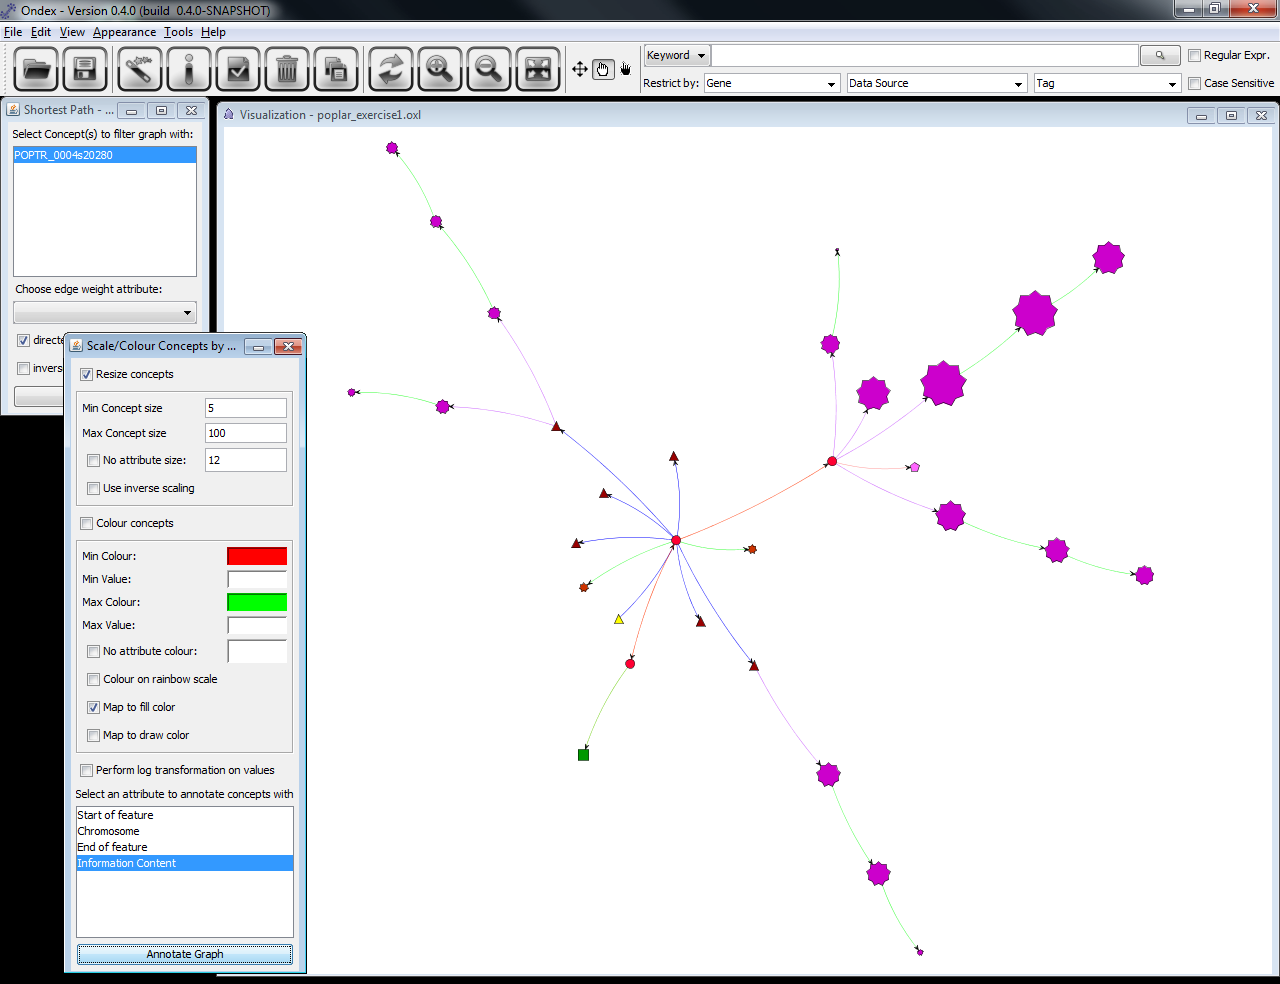
\includegraphics[scale=0.3]{images/Jun12/poplar_result_ex2_annIC.png} 
\caption{Screen-shot after annotating GO terms with their information content}
\label{fig:poplar_result_annIC}
\end{figure}

\emph{Help:}
	\begin{itemize}
	\item Hide all biological processes by clicking on one of them, right-click Hide -$>$ Same Concept Class.
	\item Apply the Gem layout again (Appearance -$>$ Layouts -$>$ Gem)
	\item Tools -$>$ Annotators -$>$ Scale/Colour Concepts by Numerical Value
	\item Select the check-box ``No attribute size'' to specify a default value for concepts which do not hold an ``Information Content'' attribute
	\item Change the sizes to 5, 100 and 5 (or experiment by yourself)
	\item Do not select ``Colour Concepts'' (we want to keep the colour as set by concept class colour legend)
	\item Select ``Information Content'' in the list of attributes available
	\item Click on ``Annotate Graph''
	\end{itemize}
\end{itemize}

%%%%%%%%%%%%%%%%%%%%%%%%%%%%%%%%%%%%%%%%%%%%%%%%%%%%%%%%%%%%%%%%%%%%%%%%%%%%%
\subsection{Exercise}
\label{sec:analysing_exercise}
Given a trait ontology term (``shoot branching'') we wish to show all Poplar proteins which are related to it in the network. 
\begin{itemize}
\item Close all the windows you have opened in Ondex (View -$>$ Windows -$>$ Close All).
\item Go to File -$>$ Open  (or click on the first button in the icon bar)
\item You should see an Open File Dialog
\item Open the Tutorial\_files/Main\_part folder, select poplar\_exercise2.oxl and click on open
\end{itemize}

\emph{Help:}
\begin{itemize}
\item Search for ``shoot branching'' in the search bar and restrict your search to the concept class ``Trait Ontology''
\item One result gets displayed. Select it and a neighbourhood depth of zero (to see only this concept), click ``Filter Graph'' and observe Figure \ref{fig:poplar_ex2_searchres}
\begin{figure}[H]
\centering
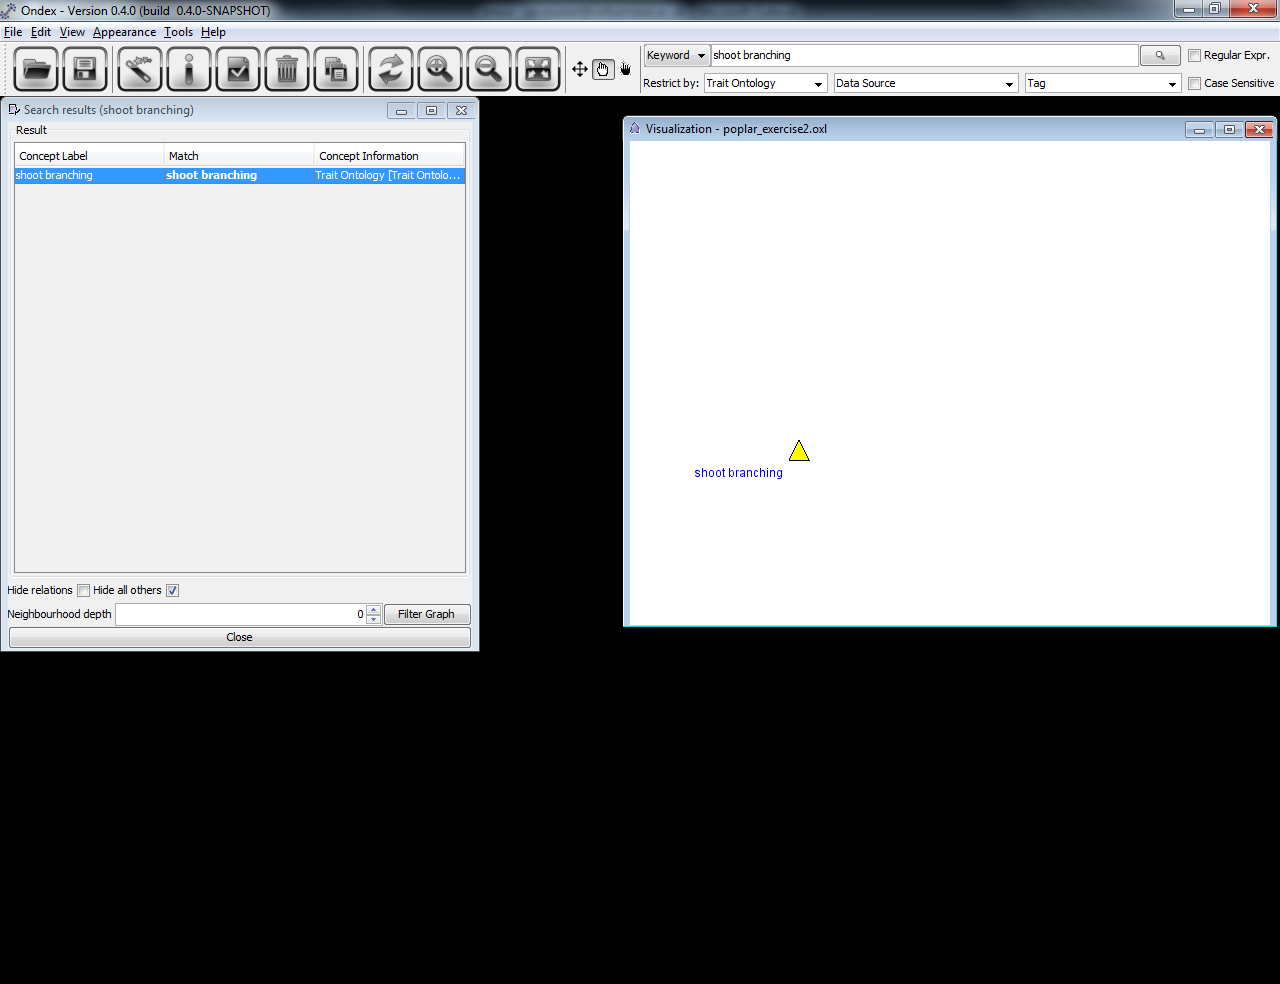
\includegraphics[scale=0.3]{images/Jun12/poplar_ex2_searchres.png} 
\caption{Screen-shot after using the embedded neighbourhood filter from the search results window}
\label{fig:poplar_ex2_searchres}
\end{figure}

\item Right-click -$>$ Show ``Immediate Neighbours by Relation Type''. 
The only one available is cooccurs\_with and will display 94 relations showing the result of the Ondex text-mining plugin (which is part of the workflow to produce this graph).
This ``shoot branching'' term cooccurs with proteins and other traits in some publications' abstracts.

\item Tools -$>$ Annotators -$>$ Scale/Colour Relations by Numerical Value
\item Select the attribute called ``Inner product of TFIDF'' in the list at the bottom
TFIDF is a measure used to evaluate how important a word is to a document in a collection or corpus (see \url{http://en.wikipedia.org/wiki/Tf-idf}).
A publication explaining the text mining module in Ondex is available at \url{http://journal.imbio.de/article.php?aid=121}.

\item Press Control A while the Visualization window is in focus to select all visible concepts in the graph
\item Right-click -$>$ Show ``Immediate Neighbours by Relation Type'' and select ``has\_similar\_sequence''
\item 91 Poplar proteins are added
\item Tools -$>$ Annotators -$>$ Scale/Colour Relations by Numerical Value
\item Tick the ``Preserve non-matching relations'' option (so that the results of the first annotator are kept)
\item Select the attribute called ``Bit Score'' in the list at the bottom
\end{itemize}

Following the cooccurs\_with relation whose width scaled up the most leads to the NCED8 (MAX4) protein in {\it{Arabidopsis}} then to POPTR\_0018s08010 and POPTR\_0006s25490 in poplar as illustrated on the screen-shot \ref{fig:poplar_ex2_searchresAnno}.
Furthermore, Ondex also offers the possibility of calling external Web services.
For example, in this case you could select these three proteins and run ClustalW using JalView.
You would need to select the three proteins, right-click -$>$ Link -$>$  Perform multiple-sequence alignment.
Once JalView is loaded up, go to Web Service -$>$ Alignment. 
\emph{Note:} other functions are available from the JalView menu ({\it{e.g.}}, calculate a phylogenetic tree).

\begin{figure}[H]
\centering
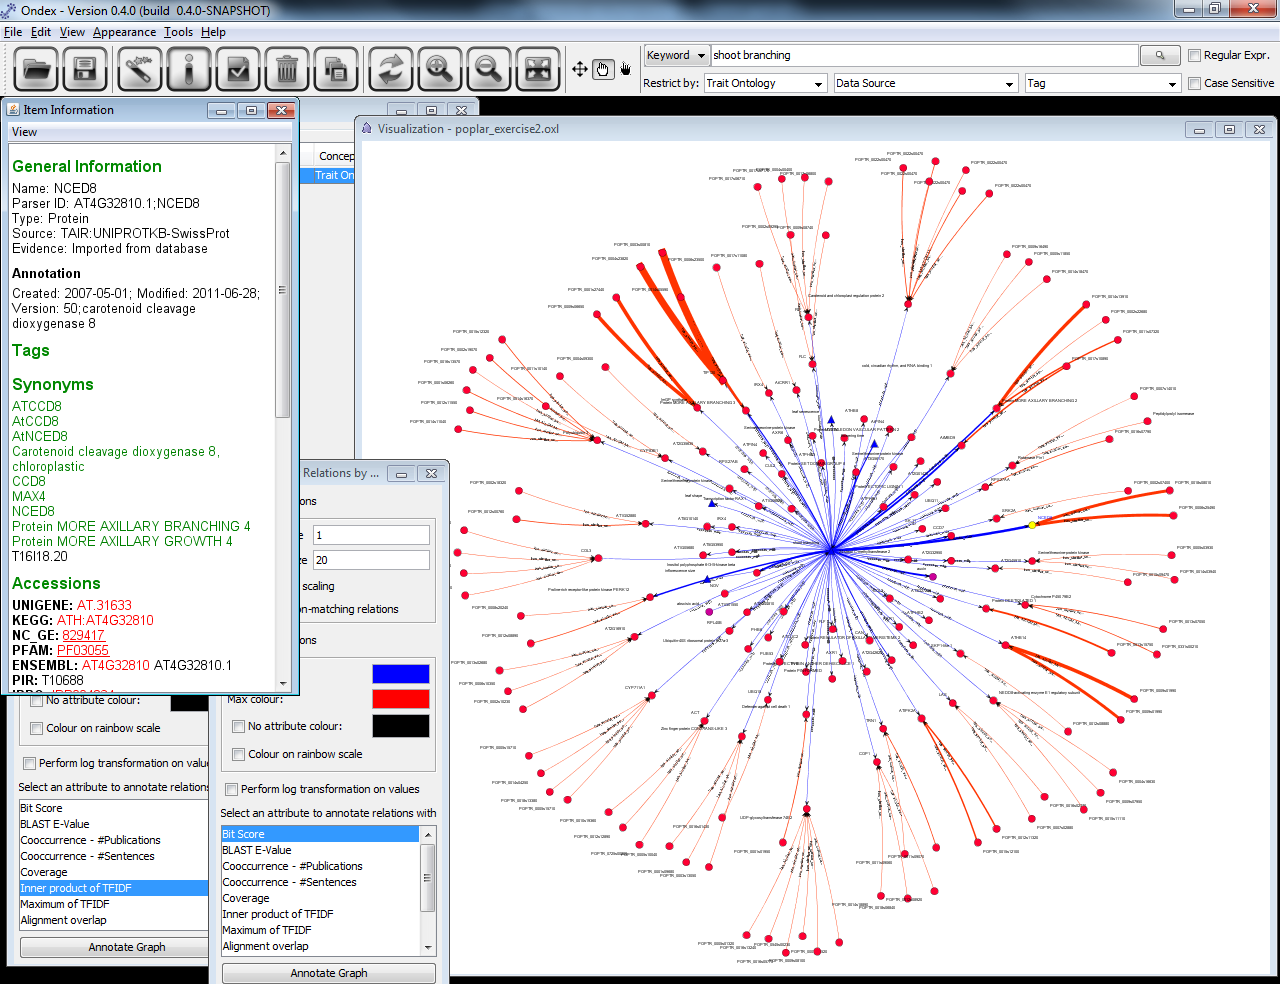
\includegraphics[scale=0.3]{images/Jun12/poplar_ex2_searchresAnno.png} 
\caption{Screen-shot after applying the Scale/Colour Relations by Numerical Value annotators}
\label{fig:poplar_ex2_searchresAnno}
\end{figure}
